\section{动量与加速}
\label{sec:fom-momentum}

上一节的结论是：病态目标上梯度下降的步数与$\kappa$成正比。不增加每步的梯度读取次数，只多用一点历史信息，能不能把这个依赖关系变小？

先看贯穿例上折返时发生了什么。图~\ref{fig:fom-zigzag}(a)把$\alpha=1/5$的每步位移分解到两个坐标。平坦方向$x_1$上，每一步的位移都向负方向，符号一致；陡峭方向$x_2$上，位移的符号每步翻转，走过去又走回来，大部分抵消。

\begin{BookInlineFigure}
  \centering
  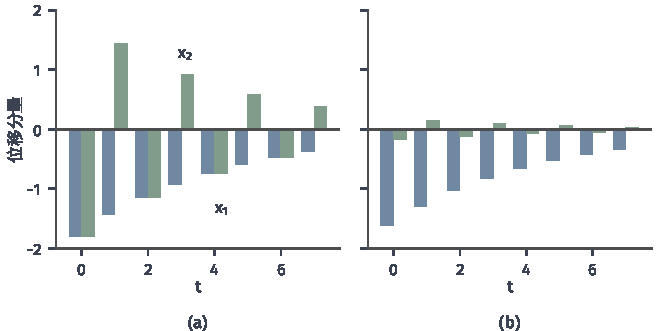
\includegraphics[width=112mm]{figures/05-optimization/02-smooth-optimization/matplotlib/fom-zigzag/figure.pdf}
  \caption{贯穿例上$\alpha=1/5$的梯度下降的位移。蓝色条是平坦方向$x_1$的分量，绿色条是陡峭方向$x_2$的分量。(a)每一步的位移$\bm{x}^{(t+1)}-\bm{x}^{(t)}$，绿色条的符号逐步交替。(b)相邻两步位移的平均，绿色条几乎消失，蓝色条保持不变的符号与相近的大小。}
  \label{fig:fom-zigzag}
\end{BookInlineFigure}

图~\ref{fig:fom-zigzag}(b)把相邻两步取平均：振荡方向互相抵消，一致方向得以保留。这就是用历史信息的线索：过去的位移本身携带了“哪些方向一直在走、哪些方向在来回”的信息，而这一信息不用额外计算梯度。

把上一步的位移乘一个系数加进当前更新，这个附加量称为\term{动量}（momentum）。下面两个方法都用动量，差别在梯度取在什么地方：重球法取在当前点，Nesterov方法取在沿动量向前试探的点。

\subsection{Polyak重球法}
\label{sec:fom-heavy-ball}

\paragraph{主要思想}
想象一个有质量的球在山谷中滚动，并受到摩擦。球的速度不会突然改变：沿谷底方向的重力持续推动，它越滚越快；沿谷壁方向的重力来回变号，速度被平均掉了。这就是想要的效果。

类比可以写成方程。位置$\bm{x}(\tau)$满足
\[
 \ddot{\bm{x}}+a\dot{\bm{x}}+\nabla f(\bm{x})=\bm{0},
\]
其中$a>0$是摩擦系数。用步长$h$的差分代替导数：
\[
 \ddot{\bm{x}}\approx\frac{\bm{x}^{(t+1)}-2\bm{x}^{(t)}+\bm{x}^{(t-1)}}{h^2},\qquad
 \dot{\bm{x}}\approx\frac{\bm{x}^{(t)}-\bm{x}^{(t-1)}}{h}.
\]

代入方程并整理，得到\term{重球法}（heavy ball method）\scite{polyak1964heavyball}：
\begin{equation}
 \bm{x}^{(t+1)}=\bm{x}^{(t)}-\alpha\bm{g}^{(t)}+\beta\bigl(\bm{x}^{(t)}-\bm{x}^{(t-1)}\bigr),
 \label{eq:fom-hb}
\end{equation}
其中$\alpha=h^2$，$\beta=1-ah$。摩擦越小，$\beta$越接近$1$，历史保留得越多。类比只解释了公式的样子，它并不提供收敛保证：离散的步子可以跨过谷底，下面会看到这确实造成困难。

$\alpha$和$\beta$怎样选？在正定二次目标上可以精确分析。与梯度下降一样，取$\bm{H}$的特征方向作坐标，由式~\eqref{eq:fom-hb}，特征值$\lambda$对应的误差分量满足二阶递推
\begin{equation}
 e_\lambda^{(t+1)}=(1+\beta-\alpha\lambda)e_\lambda^{(t)}-\beta e_\lambda^{(t-1)}.
 \label{eq:fom-hb-scalar}
\end{equation}

二阶线性递推的行为由特征方程的两个根决定：
\begin{equation}
 r^2-(1+\beta-\alpha\lambda)r+\beta=0.
 \label{eq:fom-hb-char}
\end{equation}
两根之积是$\beta$。判别式小于零时两根共轭，模相等，所以模都等于$\sqrt\beta$，\emph{与$\lambda$无关}。这是重球法最关键的现象：梯度下降的因子$1-\alpha\lambda$随方向变化，动量却可以把一段特征值的收缩速度拉平。

判别式小于等于零，就是$\lvert1+\beta-\alpha\lambda\rvert\leq2\sqrt\beta$。把它拆成上下两个不等式，并用$1+\beta\mp2\sqrt\beta=(1\mp\sqrt\beta)^2$，得到
\begin{equation}
 (1-\sqrt\beta)^2\leq\alpha\lambda\leq(1+\sqrt\beta)^2.
 \label{eq:fom-hb-complex}
\end{equation}
落在这个区间内的$\lambda$，收缩因子都是$\sqrt\beta$；落在区间外时两根是实数，积为$\beta$，其中一个的绝对值大于$\sqrt\beta$，收缩变慢。

于是设计问题变得清楚：让$[\alpha\mu,\alpha L]$全部落入区间~\eqref{eq:fom-hb-complex}，同时让$\sqrt\beta$尽量小。$\beta$越小区间越窄，所以最优时区间的两端恰好卡住，
\[
 (1-\sqrt\beta)^2=\alpha\mu,\qquad(1+\sqrt\beta)^2=\alpha L.
\]

两式开方后相除，得到$\sqrt\kappa=(1+\sqrt\beta)/(1-\sqrt\beta)$，解出$\sqrt\beta$；两式开方后相加，得到$\sqrt{\alpha L}+\sqrt{\alpha\mu}=2$，解出$\alpha$。结果是
\begin{equation}
 \alpha=\frac{4}{(\sqrt L+\sqrt\mu)^2},\qquad
 \beta=\Bigl(\frac{\sqrt\kappa-1}{\sqrt\kappa+1}\Bigr)^2.
 \label{eq:fom-hb-params}
\end{equation}
收缩因子$\sqrt\beta=(\sqrt\kappa-1)/(\sqrt\kappa+1)$的形式与梯度下降相同，只是$\kappa$换成了$\sqrt\kappa$。

例中$L=9$，$\mu=1$，$\sqrt\kappa=3$，所以
\[
 \alpha=\frac{4}{(3+1)^2}=\frac14,\qquad\beta=\Bigl(\frac24\Bigr)^2=\frac14,\qquad\sqrt\beta=\frac12.
\]

图~\ref{fig:fom-hb-roots}(a)画出$\lambda$从$1$走到$9$时根的运动。$\lambda=1$时是实轴上的二重根$\tfrac12$，随着$\lambda$增大，两根沿半径$\tfrac12$的圆分开，在$\lambda=5$时到达$\pm\tfrac12\mathrm{i}$，再在$\lambda=9$时汇合于$-\tfrac12$。梯度下降的单根则在实轴上从$0.8$移动到$-0.8$。图~\ref{fig:fom-hb-roots}(b)把模按$\lambda$展开：梯度下降是V形，重球法是平底。

\begin{BookInlineFigure}
  \centering
  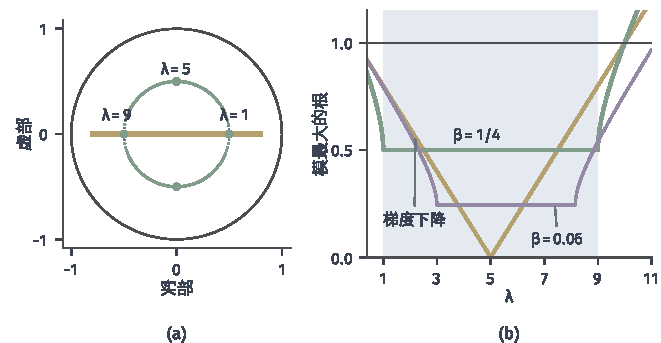
\includegraphics[width=112mm]{figures/05-optimization/02-smooth-optimization/matplotlib/fom-hb-roots/figure.pdf}
  \caption{重球法的特征根。(a)$\alpha=\beta=1/4$时，$\lambda\in[1,9]$对应的根（绿色）落在半径$1/2$的圆上；黄色线段是$\alpha=1/5$的梯度下降的根$1-\alpha\lambda$；外圈是单位圆。(b)模最大的根关于$\lambda$的变化，蓝底区间是$[\mu,L]$。绿线$\alpha=\beta=1/4$的平底宽度正好覆盖$[1,9]$；黄线是$\alpha=1/5$的梯度下降；紫线取$\alpha=0.19$，$\beta=0.06$，平底变低却变窄，靠近区间两端时被实根抬高。}
  \label{fig:fom-hb-roots}
\end{BookInlineFigure}

\needspace{6\baselineskip}
\paragraph{变量}
\begin{itemize}
 \item $\bm{x}^{(t)},\bm{x}^{(t-1)}\in\mathbb{R}^n$：当前点与上一点，比梯度下降多存一个向量。
 \item $\bm{g}^{(t)}\in\mathbb{R}^n$：当前点的梯度。
 \item $\alpha>0$，$0\leq\beta<1$：步长与动量系数，全程固定。
 \item $\varepsilon$，$T$：容差与最大步数。
\end{itemize}

\paragraph{初始化}
规定$\bm{x}^{(-1)}=\bm{x}^{(0)}$，于是第一步没有动量，就是一步梯度下降。按式~\eqref{eq:fom-hb-params}确定参数。例中$\alpha=\beta=1/4$，容差$\varepsilon=10^{-3}$，起点仍是
\[
 \bm{x}^{(-1)}=\bm{x}^{(0)}=(9,1).
\]

\needspace{6\baselineskip}
\paragraph{每轮更新}
在第$t$轮：
\begin{enumerate}
 \item \textbf{读取梯度并检查停止。}计算$\bm{g}^{(t)}$；若$\lVert\bm{g}^{(t)}\rVert_2\leq\varepsilon$或$t=T$，输出$\bm{x}^{(t)}$。例中第一轮
 \[
  \bm{g}^{(0)}=(9,9),\qquad\lVert\bm{g}^{(0)}\rVert_2\approx12.73.
 \]
 \item \textbf{计算动量项。}令$\bm{m}^{(t)}=\beta(\bm{x}^{(t)}-\bm{x}^{(t-1)})$。例中第一轮
 \[
  \bm{m}^{(0)}=\bm{0}.
 \]
 \item \textbf{更新。}按式~\eqref{eq:fom-hb}把负梯度步和动量项加到$\bm{x}^{(t)}$上，令$t\leftarrow t+1$。例中第一轮
 \[
  \bm{x}^{(1)}=(9,1)-\tfrac14(9,9)=(6.75,-1.25),\qquad f(\bm{x}^{(1)})=29.8125.
 \]

 例中第二轮，梯度和动量项分别是
 \[
  \bm{g}^{(1)}=(6.75,-11.25),\qquad\bm{m}^{(1)}=\tfrac14(-2.25,-2.25)=(-0.5625,-0.5625),
 \]
 于是
 \[
  \bm{x}^{(2)}=(6.75,-1.25)-(1.6875,-2.8125)+(-0.5625,-0.5625)=(4.5,1),
 \]
 $f(\bm{x}^{(2)})=14.625$。

 例中第三轮，梯度和动量项分别是
 \[
  \bm{g}^{(2)}=(4.5,9),\qquad\bm{m}^{(2)}=\tfrac14(-2.25,2.25)=(-0.5625,0.5625),
 \]
 于是
 \[
  \bm{x}^{(3)}=(4.5,1)-(1.125,2.25)+(-0.5625,0.5625)=(2.8125,-0.6875),
 \]
 $f(\bm{x}^{(3)})\approx6.082$。比较梯度下降的第三步$f\approx11.80$，已经差了将近一半。
\end{enumerate}

在这个例子上，式~\eqref{eq:fom-hb-char}的根是二重的：$\lambda=1$时为$\tfrac12$，$\lambda=9$时为$-\tfrac12$。二重根的递推解是$(a+bt)r^t$，由前两项定出系数，两个坐标是
\begin{equation}
 x_1^{(t)}=\frac{9+4.5t}{2^t},\qquad x_2^{(t)}=(1+1.5t)\Bigl(-\frac12\Bigr)^t.
 \label{eq:fom-hb-closed}
\end{equation}

代入$t=19$，梯度大小约为$5.4\times10^{-4}$，$t=18$时仍大于$10^{-3}$，于是第$19$步满足容差并结束。最终得到
\[
 \bm{x}^{(19)}\approx(1.80\times10^{-4},\,-5.63\times10^{-5}).
\]
同样的容差，梯度下降$\alpha=1/5$需要$43$步。

\paragraph{二次目标上的收敛}
式~\eqref{eq:fom-hb-closed}中的$1+1.5t$值得留意：根是二重时，收敛并不是纯粹的$\rho^t$，前面还有一个线性增长的因子。下面的定理把它显式写出来。

\begin{theorem}[正定二次目标上的重球法]
\label{thm:fom-hb-quadratic}
设$f$是Hessian为$\bm{H}$的二次目标，最优解为$\bm{x}^\star$，$\bm{H}$对称正定，特征值落在$[\mu,L]$内，$\kappa=L/\mu>1$。按式~\eqref{eq:fom-hb-params}取参数，令$\bm{x}^{(-1)}=\bm{x}^{(0)}$，$\rho=(\sqrt\kappa-1)/(\sqrt\kappa+1)$，则
\begin{equation}
 \lVert\bm{x}^{(t)}-\bm{x}^\star\rVert_2\leq(2t+1)\rho^t\lVert\bm{x}^{(0)}-\bm{x}^\star\rVert_2.
 \label{eq:fom-hb-rate}
\end{equation}
\end{theorem}

\begin{proof}
由式~\eqref{eq:fom-hb-complex}及参数的取法，每个特征值对应的两根$r_1,r_2$的模都等于$\rho$，并且$r_1+r_2=1+\beta-\alpha\lambda$，$r_1r_2=\beta=\rho^2$。

定义$S_k=\sum_{j=0}^kr_1^jr_2^{k-j}$，规定$S_{-1}=0$。由定义有$S_{k+1}=r_1S_k+r_2^{k+1}$，同理$S_k=r_1S_{k-1}+r_2^k$。把第二式乘以$r_2$后代入第一式，得到
\[
 S_{k+1}=(r_1+r_2)S_k-r_1r_2S_{k-1}.
\]

所以$S_t$满足递推~\eqref{eq:fom-hb-scalar}。分量的解可以写成$e^{(t)}=S_te^{(0)}-\beta S_{t-1}e^{(-1)}$：它满足同一递推，而$t=0$和$t=1$时分别等于$e^{(0)}$和式~\eqref{eq:fom-hb-scalar}的右端。

由$e^{(-1)}=e^{(0)}$，$\lvert S_k\rvert\leq(k+1)\rho^k$和$\beta=\rho^2$，
\[
 \lvert e^{(t)}\rvert\leq\bigl((t+1)\rho^t+\rho^2\,t\,\rho^{t-1}\bigr)\lvert e^{(0)}\rvert\leq(2t+1)\rho^t\lvert e^{(0)}\rvert,
\]
最后一步用了$\rho<1$。对所有特征方向平方求和，再用标准正交变换保持长度，即得结论。
\end{proof}

证明中间一步的界是$(t+1+\rho t)\rho^t$。例中$\rho=\tfrac12$，第二坐标恰好取到这个界，即$(1+1.5t)2^{-t}$，与式~\eqref{eq:fom-hb-closed}相符。图~\ref{fig:fom-hb-paths}(b)展示了多项式因子的后果：比值$x_2^{(t)}/x_2^{(0)}$第一步到达$-1.25$，比初值还大，随后才在紫色包络线外侧逐渐衰减。

\begin{BookInlineFigure}
  \centering
  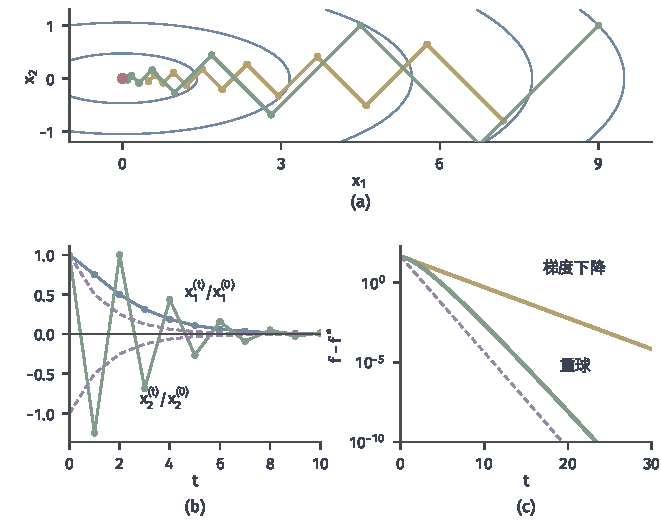
\includegraphics[width=112mm]{figures/05-optimization/02-smooth-optimization/matplotlib/fom-hb-paths/figure.pdf}
  \caption{贯穿例上的重球法（绿色，$\alpha=\beta=1/4$）与梯度下降（黄色，$\alpha=1/5$）。(a)等高线上的前$14$步。(b)重球法两坐标相对初值的比，式~\eqref{eq:fom-hb-closed}，紫色虚线是$\pm\rho^t$。(c)目标差的半对数曲线，紫色虚线是$45\rho^{2t}$，绿线在上方平行，差别来自多项式因子。}
  \label{fig:fom-hb-paths}
\end{BookInlineFigure}

所以，用$\rho$比较两种方法时，要记住它是渐近的说法。达到相对精度$\varepsilon$的步数约为$\tfrac{\sqrt\kappa}{2}\ln(1/\varepsilon)$，与梯度下降的$\tfrac\kappa2\ln(1/\varepsilon)$相比，$\kappa=10^4$时大约快一百倍。

\paragraph{参数的稳定范围}
这个加速依赖于参数对$L$和$\mu$的准确了解。由递推~\eqref{eq:fom-hb-scalar}的两根都在单位圆内的条件，可以写出稳定范围。多项式$p(r)=r^2-(1+\beta-\alpha\lambda)r+\beta$满足$p(1)=\alpha\lambda$，$p(-1)=2(1+\beta)-\alpha\lambda$，在$\beta\geq0$时，两根都在单位圆内当且仅当
\begin{equation}
 \beta<1,\qquad0<\alpha\lambda<2(1+\beta).
 \label{eq:fom-hb-stable}
\end{equation}

判据是$p(1)>0$，$p(-1)>0$，且根之积$\beta$的绝对值小于$1$。例中若沿用$\alpha=1/4$，却把$\beta$减到$0.06$，则$\alpha L=2.25$大于$2(1+\beta)=2.12$，陡峭方向发散。动量不只是“加速的旋钮”，它也放宽了步长的稳定界限，两个参数必须一起调。

\paragraph{离开二次目标}
式~\eqref{eq:fom-hb-params}的推导完全依赖于每个方向有固定的$\lambda$。目标不是二次时，局部曲率随位置变化，没有固定的特征方向。若$f$二阶连续可微，而$\bm{x}^\star$处的Hessian特征值落在$[\mu,L]$内，在$\bm{x}^\star$足够近处迭代可以用线性化来分析，局部收敛速度接近$\rho$；这是局部结论，对起点有要求。

全局情形下，这组参数确实可能失败。考虑一元函数，其导数分三段：
\begin{equation}
 f'(x)=\begin{cases}
 25x,&x<1,\\
 x+24,&1\leq x<2,\\
 25x-24,&x\geq2.
 \end{cases}
 \label{eq:fom-hb-counterexample}
\end{equation}
三段在分界点处衔接，$f'$连续且斜率都在$[1,25]$内，所以$f$强凸，$\mu=1$，$L=25$，最优解是$x^\star=0$。二次目标的最优参数是$\alpha=1/9$，$\beta=4/9$。

这组参数有一个周期为$3$的轨道，不会收敛：
\[
 x\text{ 依次取}\quad \frac{792}{1225},\quad-\frac{2208}{1225},\quad\frac{2592}{1225}.
\]

可以逐步核对。从前两点$2592/1225$（上一点）和$792/1225$（当前点）出发，当前点小于$1$，导数是$25x$。代入式~\eqref{eq:fom-hb}并把分母提出来：
\[
 x^{+}=\frac{1}{1225}\Bigl(792-\frac{25\cdot792}{9}+\frac49(792-2592)\Bigr)=-\frac{2208}{1225}.
\]

下一步当前点$-2208/1225$仍小于$1$，同样算得$2592/1225$。再下一步，当前点约为$2.116$，落在第三段，导数$25x-24$多出的常数$-24$提供了回拉，算得的新点恰好回到$792/1225$。

图~\ref{fig:fom-hb-cycle}展示了$x^{(0)}=3.3$时的情形：迭代很快落到这个周期上。作为对照，下一小节的方法在同一函数上正常收敛。这个反例说明，正定二次目标上的最优参数不能直接移到一般强凸目标上，也不能因此宣称全局加速。

\begin{BookInlineFigure}
  \centering
  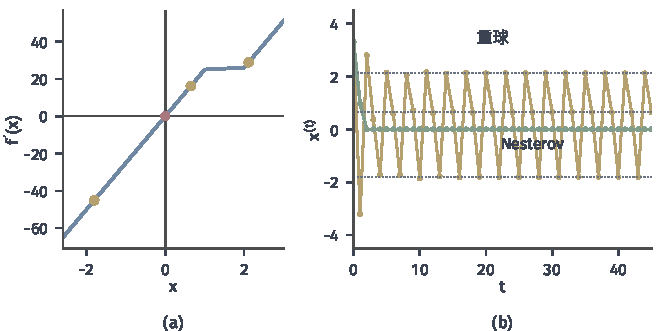
\includegraphics[width=112mm]{figures/05-optimization/02-smooth-optimization/matplotlib/fom-hb-cycle/figure.pdf}
  \caption{强凸光滑目标上重球法不收敛的例子。(a)式~\eqref{eq:fom-hb-counterexample}的导数$f'(x)$（蓝线），红点是最优解，黄点是周期轨道的三个点。(b)从$x^{(0)}=3.3$出发的迭代，黄线是重球法（$\alpha=1/9$，$\beta=4/9$），落到灰色点线标出的周期上；绿线是$\alpha=1/25$，$\beta=2/3$的Nesterov方法，收敛到$0$。}
  \label{fig:fom-hb-cycle}
\end{BookInlineFigure}

对一般强凸目标，缩小参数可以恢复全局收敛，但已知的这类分析一般达不到$\sqrt\kappa$的依赖，具体的条件和常数需要逐项核对，证明较长，读者可查阅一阶方法的专门文献。本章只在正定二次目标上给重球法下定量结论。

\subsection{Nesterov加速梯度法}
\label{sec:fom-nesterov}

\paragraph{主要思想}
重球法的动量盲目地累加：梯度在当前点读取，动量推出的位置却没有被检查，步子跨过谷底时也不会被纠正。一个自然的改进是把两件事的次序换一下：先顺着动量探出去，到探出的位置上再看坡度，用那里的梯度来修正。

这就是\term{Nesterov加速梯度法}（Nesterov accelerated gradient）\scite{nesterov1983method}。

它先由当前与历史迭代构成\term{外推点}（extrapolation point）$\bm{y}^{(t)}$，再在外推点做一步梯度下降：
\begin{equation}
 \begin{aligned}
 \bm{y}^{(t)}&=\bm{x}^{(t)}+\beta^{(t)}\bigl(\bm{x}^{(t)}-\bm{x}^{(t-1)}\bigr),\\
 \bm{x}^{(t+1)}&=\bm{y}^{(t)}-\alpha\nabla f(\bm{y}^{(t)}).
 \end{aligned}
 \label{eq:fom-nag}
\end{equation}
与式~\eqref{eq:fom-hb}比较，只有梯度的计算位置不同。图~\ref{fig:fom-nag-geometry}把一步的结构并排画出。

\begin{BookInlineFigure}
  \centering
  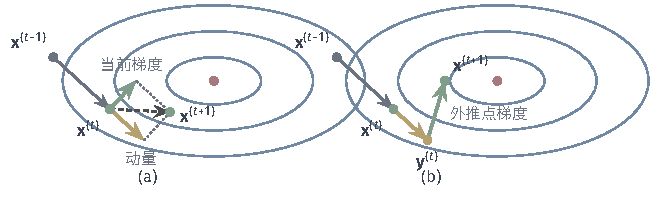
\includegraphics[width=110mm]{figures/05-optimization/02-smooth-optimization/tikz/fom-nag-geometry/figure.pdf}
  \caption{一步更新的结构对比，蓝色椭圆是等高线，红点是最优解。(a)重球法：动量（黄）和当前点的负梯度（绿）都从$\bm{x}^{(t)}$出发，两者相加得到新点。(b)Nesterov方法：先沿动量走到外推点$\bm{y}^{(t)}$，再从那里走一步负梯度。外推点已经冲到谷壁的外侧，那里的梯度把步子拉回。}
  \label{fig:fom-nag-geometry}
\end{BookInlineFigure}

用二次目标看这一改变的效果。代入$\nabla f(\bm{y})=\bm{H}(\bm{y}-\bm{x}^\star)$，并在特征方向上写开，记$s=1-\alpha\lambda$，得到
\begin{equation}
 e_\lambda^{(t+1)}=s\Bigl((1+\beta)e_\lambda^{(t)}-\beta e_\lambda^{(t-1)}\Bigr).
 \label{eq:fom-nag-scalar}
\end{equation}

对照式~\eqref{eq:fom-hb-scalar}。重球法的$-\beta e^{(t-1)}$不受$\lambda$影响，动量对各方向一视同仁；这里动量也被乘了$s$，曲率大的方向$s$小，动量被自动压低。这就是“外推点的梯度纠正动量”在公式上的含义。

特征方程是$r^2-s(1+\beta)r+s\beta=0$。复根时两根的积等于模的平方，所以模是$\sqrt{s\beta}$，随$\lambda$的增大而减小。

参数怎样选？取$\alpha=1/L$。例如强凸时取
\begin{equation}
 \beta=\frac{\sqrt\kappa-1}{\sqrt\kappa+1}.
 \label{eq:fom-nag-beta-strong}
\end{equation}
于是最平坦的方向$\lambda=\mu$上，$s=1-1/\kappa$，判别式恰好为零，二重根是$1-1/\sqrt\kappa$。由$(1+\beta)^2s=4\beta$可以直接验证这一点：把$\beta$代入，$(1+\beta)=2\sqrt\kappa/(\sqrt\kappa+1)$，$4\beta/(1+\beta)^2=(\kappa-1)/\kappa=s$。

而光滑凸时，$\mu$不可用，系数要随步数增长，后文的定理将说明它的具体形式。例中$\sqrt\kappa=3$，
\[
 \alpha=\frac19,\qquad\beta=\frac12,\qquad1-\frac{1}{\sqrt\kappa}=\frac23.
\]

\needspace{6\baselineskip}
\paragraph{变量}
\begin{itemize}
 \item $\bm{x}^{(t)},\bm{x}^{(t-1)}\in\mathbb{R}^n$：当前点与上一点。
 \item $\bm{y}^{(t)}\in\mathbb{R}^n$：外推点，梯度在这里读取，用后可覆盖。
 \item $\alpha$，$\beta^{(t)}$：步长和外推系数。
 \item $\varepsilon$，$T$：容差与最大步数。
\end{itemize}

\paragraph{初始化}
令$\bm{x}^{(-1)}=\bm{x}^{(0)}$，于是$\bm{y}^{(0)}=\bm{x}^{(0)}$。例中$\alpha=1/9$，$\beta=1/2$，容差$\varepsilon=10^{-3}$，
\[
 \bm{y}^{(0)}=\bm{x}^{(0)}=(9,1).
\]

\needspace{6\baselineskip}
\paragraph{每轮更新}
在第$t$轮：
\begin{enumerate}
 \item \textbf{外推。}由式~\eqref{eq:fom-nag}的第一行计算$\bm{y}^{(t)}$。例中第一轮
 \[
  \bm{y}^{(0)}=(9,1).
 \]
 \item \textbf{读取外推点梯度并更新。}由式~\eqref{eq:fom-nag}的第二行计算$\bm{x}^{(t+1)}$。例中第一轮
 \[
  \nabla f(\bm{y}^{(0)})=(9,9),\qquad\bm{x}^{(1)}=(9,1)-\tfrac19(9,9)=(8,0).
 \]

 例中第二轮的外推点和梯度是
 \[
  \bm{y}^{(1)}=(8,0)+\tfrac12(-1,-1)=(7.5,-0.5),\qquad\nabla f(\bm{y}^{(1)})=(7.5,-4.5),
 \]
 于是
 \[
  \bm{x}^{(2)}=(7.5,-0.5)-\tfrac19(7.5,-4.5)=\bigl(\tfrac{20}3,0\bigr).
 \]

 例中第三轮的外推点和梯度是
 \[
  \bm{y}^{(2)}=\bigl(\tfrac{20}3,0\bigr)+\tfrac12\bigl(-\tfrac43,0\bigr)=(6,0),\qquad\nabla f(\bm{y}^{(2)})=(6,0),
 \]
 于是
 \[
  \bm{x}^{(3)}=(6,0)-\tfrac19(6,0)=\bigl(\tfrac{16}3,0\bigr).
 \]
 \item \textbf{检查停止。}若新点的梯度大小不超过$\varepsilon$或已达$T$步，输出$\bm{x}^{(t+1)}$。这一检查要在$\bm{x}^{(t+1)}$处多读一次梯度，实际计算中常改用外推点的梯度大小，或每隔若干步才检查。例中第三轮$\lVert\nabla f(\bm{x}^{(3)})\rVert_2\approx5.33$，继续。
\end{enumerate}

例中第二坐标在第一步之后就是零，原因是陡峭方向$\lambda=L$上$s=0$，由式~\eqref{eq:fom-nag-scalar}，下一步的误差直接等于零。平坦方向的递推是$e^{(t+1)}=\tfrac43e^{(t)}-\tfrac49e^{(t-1)}$，二重根是$\tfrac23$，解出
\begin{equation}
 x_1^{(t)}=(9+3t)\Bigl(\frac23\Bigr)^t,\qquad x_2^{(t)}=0\quad(t\geq1).
 \label{eq:fom-nag-closed}
\end{equation}

代入式~\eqref{eq:fom-nag-closed}，第$29$步首次满足容差。最终得到
\[
 \bm{x}^{(29)}\approx(7.51\times10^{-4},\,0).
\]

\paragraph{强凸情形的势函数分析}
图~\ref{fig:fom-nag-paths}(b)比较了三种方法在例中各方向上的根，(c)是目标差。在这个二次例子上，重球法的因子$\tfrac12$比Nesterov方法的$\tfrac23$更小，步数$19$也少于$29$。Nesterov方法的价值不在于二次目标上最快，而在于它的保证可以一直延伸到一般的强凸光滑目标，而这正是重球法在式~\eqref{eq:fom-hb-counterexample}中失败的地方。

\begin{BookInlineFigure}
  \centering
  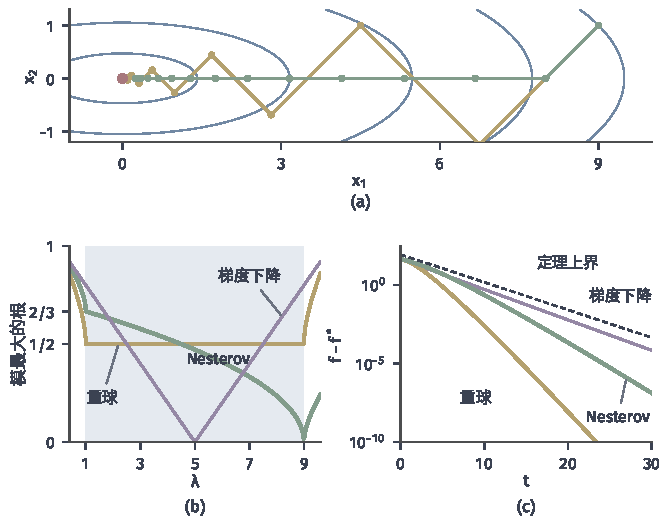
\includegraphics[width=112mm]{figures/05-optimization/02-smooth-optimization/matplotlib/fom-nag-paths/figure.pdf}
  \caption{贯穿例上的Nesterov方法（绿色，$\alpha=1/9$，$\beta=1/2$），对照重球法（黄色，$\alpha=\beta=1/4$）和梯度下降（紫色，$\alpha=1/5$）。(a)等高线上的前$14$步。(b)模最大的根关于$\lambda$的变化，蓝底区间是$[\mu,L]$。(c)目标差，黑色虚线是式~\eqref{eq:fom-nag-strong}给出的上界$86(2/3)^t$。}
  \label{fig:fom-nag-paths}
\end{BookInlineFigure}

要在一般目标上证明收敛，不能再用特征分解，也不能指望函数值单调下降：动量可能把函数值暂时抬高。需要另找一个每步都下降的量，称为\term{势函数}（potential function）。它把“函数值的差”和“某个辅助点到解的距离”加起来，走动时一项增大可以由另一项吸收。

设$q=1/\sqrt\kappa=\sqrt{\mu/L}$，引入辅助点序列$\bm{v}^{(0)}=\bm{x}^{(0)}$，
\begin{equation}
 \bm{v}^{(t+1)}=\bm{x}^{(t)}+\frac1q\bigl(\bm{x}^{(t+1)}-\bm{x}^{(t)}\bigr).
 \label{eq:fom-nag-v}
\end{equation}
它是沿本步位移放大$1/q$倍得到的“更大胆的点”。

\begin{theorem}[强凸情形的Nesterov方法]
\label{thm:fom-nag-strong}
设$f$的梯度$L$-Lipschitz连续且$\mu$强凸，$\mu>0$。取$\alpha=1/L$和式~\eqref{eq:fom-nag-beta-strong}的常数$\beta$，$\bm{x}^{(-1)}=\bm{x}^{(0)}$。则势函数
\begin{equation}
 \Phi^{(t)}=f(\bm{x}^{(t)})-f^\star+\frac\mu2\lVert\bm{v}^{(t)}-\bm{x}^\star\rVert_2^2
 \label{eq:fom-nag-potential}
\end{equation}
满足$\Phi^{(t+1)}\leq(1-1/\sqrt\kappa)\Phi^{(t)}$，因此
\begin{equation}
 f(\bm{x}^{(T)})-f^\star\leq\Bigl(1-\frac{1}{\sqrt\kappa}\Bigr)^T\Bigl(f(\bm{x}^{(0)})-f^\star+\frac\mu2\lVert\bm{x}^{(0)}-\bm{x}^\star\rVert_2^2\Bigr).
 \label{eq:fom-nag-strong}
\end{equation}
\end{theorem}

\begin{proof}
固定一步，省略上标$(t)$，记$\bm{g}=\nabla f(\bm{y})$，$\bm{x}^+$和$\bm{v}^+$为下一步的点。先把辅助点写成便于计算的形式。

第一步，验证两个恒等式：
\[
 \bm{y}=\frac{\bm{x}+q\bm{v}}{1+q},\qquad
 \bm{v}^+=(1-q)\bm{v}+q\bm{y}-\frac q\mu\bm{g}.
\]

第一式在$t=0$时成立。设它对$t$成立，则$q\bm{v}=(1+q)\bm{y}-\bm{x}$，代入第二式右端，并用$\frac{q}{\mu}=\frac{1}{qL}$和$\bm{x}^+=\bm{y}-\bm{g}/L$，化简得到
\[
 \frac1q\bigl(\bm{x}^+-(1-q)\bm{x}\bigr)=\bm{x}+\frac1q(\bm{x}^+-\bm{x}),
\]
正是式~\eqref{eq:fom-nag-v}。再把$\bm{v}^+$代入$(\bm{x}^++q\bm{v}^+)/(1+q)$，得到
\[
 \bm{x}^++\frac{1-q}{1+q}(\bm{x}^+-\bm{x})=\bm{y}^{(t+1)},
\]
所以第一式对$t+1$成立；这里用到$\beta=(1-q)/(1+q)$，它就是式~\eqref{eq:fom-nag-beta-strong}。

第二步，估计距离项。记$\bm{w}=(1-q)\bm{v}+q\bm{y}$，则$\bm{v}^+=\bm{w}-\frac q\mu\bm{g}$，展开平方并乘$\frac\mu2$：
\[
 \frac\mu2\lVert\bm{v}^+-\bm{x}^\star\rVert_2^2
 =\frac\mu2\lVert\bm{w}-\bm{x}^\star\rVert_2^2-q\bm{g}^\top(\bm{w}-\bm{x}^\star)+\frac{q^2}{2\mu}\lVert\bm{g}\rVert_2^2.
\]

第三步，函数项。由下降引理，外推点走一步满足
\[
 f(\bm{x}^+)\leq f(\bm{y})-\frac{1}{2L}\lVert\bm{g}\rVert_2^2.
\]

又$q^2/(2\mu)=1/(2L)$，两边的$\lVert\bm{g}\rVert_2^2$恰好抵消。再用平方范数的凸性拆开$\bm{w}$，得到
\[
 \Phi^{(t+1)}\leq f(\bm{y})-f^\star+(1-q)\frac\mu2\lVert\bm{v}-\bm{x}^\star\rVert_2^2+q\frac\mu2\lVert\bm{y}-\bm{x}^\star\rVert_2^2-q\bm{g}^\top(\bm{w}-\bm{x}^\star).
\]

第四步，处理内积。把$\bm{w}-\bm{x}^\star$拆开：
\[
 \bm{w}-\bm{x}^\star=(1-q)(\bm{v}-\bm{y})+(\bm{y}-\bm{x}^\star).
\]

对后一部分用强凸性：
\[
 q\bm{g}^\top(\bm{y}-\bm{x}^\star)\geq q\bigl(f(\bm{y})-f^\star\bigr)+q\frac\mu2\lVert\bm{y}-\bm{x}^\star\rVert_2^2.
\]
代入后，$\lVert\bm{y}-\bm{x}^\star\rVert_2^2$项抵消，留下
\[
 \Phi^{(t+1)}\leq(1-q)\bigl(f(\bm{y})-f^\star\bigr)+(1-q)\frac\mu2\lVert\bm{v}-\bm{x}^\star\rVert_2^2-q(1-q)\bm{g}^\top(\bm{v}-\bm{y}).
\]

第五步，由第一式$q(\bm{v}-\bm{y})=\bm{y}-\bm{x}$，末项等于$(1-q)\bm{g}^\top(\bm{x}-\bm{y})$。凸性给出
\[
 \bm{g}^\top(\bm{x}-\bm{y})\leq f(\bm{x})-f(\bm{y}),
\]
于是$f(\bm{y})$消去，
\[
 \Phi^{(t+1)}\leq(1-q)\Bigl(f(\bm{x})-f^\star+\frac\mu2\lVert\bm{v}-\bm{x}^\star\rVert_2^2\Bigr)=(1-q)\Phi^{(t)}.
\]

由$\bm{v}^{(0)}=\bm{x}^{(0)}$，迭代得
\[
 f(\bm{x}^{(T)})-f^\star\leq\Phi^{(T)}\leq(1-q)^T\Phi^{(0)}.
\]
\end{proof}

用贯穿例核对势函数。$\mu=1$，$q=\tfrac13$，辅助点由式~\eqref{eq:fom-nag-v}算出，三个势函数值依次是
\[
 \begin{aligned}
 \bm{v}^{(0)}&=(9,1), &\Phi^{(0)}&=45+41=86,\\
 \bm{v}^{(1)}&=(6,-2), &\Phi^{(1)}&=32+20=52,\\
 \bm{v}^{(2)}&=(4,0), &\Phi^{(2)}&\approx22.22+8=30.22.
 \end{aligned}
\]
定理要求每步至少缩小到$\tfrac23$：$86\cdot\tfrac23\approx57.3\geq52$，$52\cdot\tfrac23\approx34.7\geq30.22$。

强凸性给出距离项不超过初始目标差，所以式~\eqref{eq:fom-nag-strong}右端不超过初始目标差的$2(1-1/\sqrt\kappa)^T$倍。所以达到目标差$\varepsilon$的步数约为$\sqrt\kappa\ln(1/\varepsilon)$，与重球法在二次目标上的量级相同，但条件只要求一般的强凸光滑。式~\eqref{eq:fom-hb-counterexample}满足这些条件，定理保证了图~\ref{fig:fom-hb-cycle}中绿线的收敛。

\paragraph{光滑凸情形的势函数分析}
没有强凸常数时，常数的$\beta$无从定义。这时让外推系数随步数增长。定义
\begin{equation}
 \theta^{(0)}=1,\qquad\theta^{(t+1)}=\frac{1+\sqrt{1+4(\theta^{(t)})^2}}{2},\qquad
 \beta^{(t+1)}=\frac{\theta^{(t)}-1}{\theta^{(t+1)}},
 \label{eq:fom-nag-theta}
\end{equation}
并取$\beta^{(0)}=0$，$\alpha=1/L$。$\theta^{(t+1)}$是方程$\theta^2-\theta=(\theta^{(t)})^2$的正根，这个关系在证明中恰好让相邻两项抵消。由$\theta^{(t+1)}\geq\theta^{(t)}+\tfrac12$得$\theta^{(t)}\geq(t+2)/2$，系数$\beta^{(t)}$逐步趋近于$1$。

\begin{theorem}[光滑凸情形的Nesterov方法]
\label{thm:fom-nag-convex}
设$f$凸，梯度$L$-Lipschitz连续，存在最优解$\bm{x}^\star$。按式~\eqref{eq:fom-nag}、\eqref{eq:fom-nag-theta}迭代，$\alpha=1/L$，则对任意$T\geq1$，
\begin{equation}
 f(\bm{x}^{(T)})-f^\star\leq\frac{2L\lVert\bm{x}^{(0)}-\bm{x}^\star\rVert_2^2}{(T+1)^2}.
 \label{eq:fom-nag-convex}
\end{equation}
\end{theorem}

\begin{proof}
第一步，建立一个单步不等式。设$\bm{y}$任意，$\bm{x}^+=\bm{y}-\nabla f(\bm{y})/L$，$\bm{z}$任意。由下降引理和凸性，
\[
 f(\bm{x}^+)\leq f(\bm{z})+\nabla f(\bm{y})^\top(\bm{y}-\bm{z})-\frac{1}{2L}\lVert\nabla f(\bm{y})\rVert_2^2.
\]

把$\nabla f(\bm{y})=L(\bm{y}-\bm{x}^+)$代入，并用恒等式
\[
 2\bm{a}^\top\bm{b}-\lVert\bm{a}\rVert_2^2=\lVert\bm{b}\rVert_2^2-\lVert\bm{b}-\bm{a}\rVert_2^2,
\]
其中$\bm{a}=\bm{y}-\bm{x}^+$，$\bm{b}=\bm{y}-\bm{z}$，得到
\begin{equation}
 f(\bm{x}^+)-f(\bm{z})\leq\frac L2\Bigl(\lVert\bm{y}-\bm{z}\rVert_2^2-\lVert\bm{x}^+-\bm{z}\rVert_2^2\Bigr).
 \label{eq:fom-nag-one-step}
\end{equation}

第二步，选择比较点。省略上标$(t)$，记$\theta=\theta^{(t)}$，$\Delta_t=f(\bm{x}^{(t)})-f^\star$。取
\[
 \bm{z}=\Bigl(1-\frac1\theta\Bigr)\bm{x}+\frac1\theta\bm{x}^\star.
\]

由凸性，
\[
 f(\bm{z})-f^\star\leq\Bigl(1-\frac1\theta\Bigr)\Delta_t.
\]

代入式~\eqref{eq:fom-nag-one-step}，两边乘以$\theta^2$，把$\theta$乘进范数：
\[
 \theta^2\Delta_{t+1}-(\theta^2-\theta)\Delta_t\leq\frac L2\Bigl(\lVert\theta\bm{y}-\theta\bm{z}\rVert_2^2-\lVert\theta\bm{x}^+-\theta\bm{z}\rVert_2^2\Bigr).
\]

第三步，识别辅助点。令
\[
 \bm{v}^{(t)}=\theta^{(t)}\bm{y}^{(t)}-\bigl(\theta^{(t)}-1\bigr)\bm{x}^{(t)},
\]
于是
\[
 \theta\bm{y}-\theta\bm{z}=\bm{v}^{(t)}-\bm{x}^\star.
\]

而由式~\eqref{eq:fom-nag}和式~\eqref{eq:fom-nag-theta}，$\theta^{(t+1)}\bm{y}^{(t+1)}$可以写开，得到
\[
 \bm{v}^{(t+1)}=\bm{x}^{(t)}+\theta^{(t)}\bigl(\bm{x}^{(t+1)}-\bm{x}^{(t)}\bigr),
\]
这恰好是$\theta\bm{x}^+-\theta\bm{z}+\bm{x}^\star$。

第四步，定义势函数$E^{(t)}$并裂项。规定$\theta^{(-1)}=0$，令
\[
 E^{(t)}=\bigl(\theta^{(t-1)}\bigr)^2\Delta_t+\frac L2\lVert\bm{v}^{(t)}-\bm{x}^\star\rVert_2^2.
\]

由$\theta^2-\theta=(\theta^{(t-1)})^2$（$t=0$时两边都是零），上一步的不等式就是$E^{(t+1)}\leq E^{(t)}$。又$\bm{v}^{(0)}=\bm{x}^{(0)}$，所以
\[
 \bigl(\theta^{(T-1)}\bigr)^2\Delta_T\leq E^{(T)}\leq E^{(0)}=\frac L2\lVert\bm{x}^{(0)}-\bm{x}^\star\rVert_2^2.
\]

再用$\theta^{(T-1)}\geq(T+1)/2$，即得式~\eqref{eq:fom-nag-convex}。
\end{proof}

$1/T$变成了$1/T^2$。目标差要达到$\varepsilon$，步数从$LR^2/(2\varepsilon)$降到约$\sqrt{2L/\varepsilon}\,R$。图~\ref{fig:fom-nag-convex}(a)用一个三对角的二次函数验证这一点，它的特征值一路逼近零，强凸常数实际上帮不上忙。

\begin{BookInlineFigure}
  \centering
  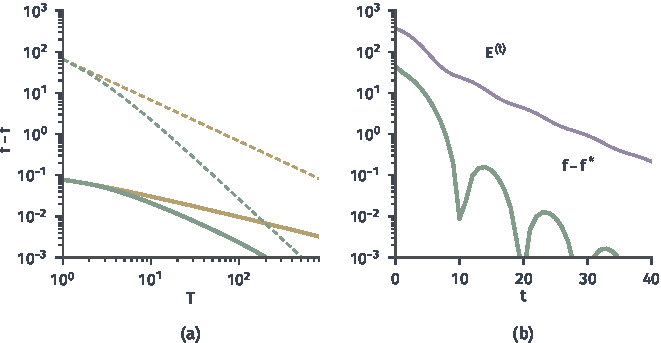
\includegraphics[width=112mm]{figures/05-optimization/02-smooth-optimization/matplotlib/fom-nag-convex/figure.pdf}
  \caption{光滑凸目标上的$1/T$与$1/T^2$。(a)$f(\bm{x})=\tfrac14(\tfrac12\bm{x}^\top\bm{A}\bm{x}-x_1)$，$\bm{A}$是$400$阶三对角矩阵（对角元$2$，次对角元$-1$），$L=1$，$\bm{x}^{(0)}=\bm{0}$。黄线是梯度下降，绿线是Nesterov方法（$\theta$形式），同色虚线是式~\eqref{eq:fom-gd-convex}、\eqref{eq:fom-nag-convex}的上界。(b)贯穿例按$\theta$形式运行，$L=9$：绿线是目标差，出现回升；紫线是势函数$E^{(t)}$，逐步下降。}
  \label{fig:fom-nag-convex}
\end{BookInlineFigure}

图~\ref{fig:fom-nag-convex}(b)说明势函数的用意。贯穿例按式~\eqref{eq:fom-nag-theta}的参数运行时，$\beta^{(t)}$逐渐接近$1$，动量过大，目标差出现$13$次回升，而$E^{(t)}$从$369$（$t=0$）、$320$（$t=1$）一路下降。凸情形的结论控制的是最后一步的目标差上界，并没有说目标差单调下降。

可以用势函数检查第一步的计算：由$\theta^{(0)}=1$得$\bm{v}^{(1)}=\bm{x}^{(1)}=(8,0)$，所以
\[
 E^{(1)}=1\cdot32+\frac92\cdot64=320,\qquad E^{(0)}=\frac92\cdot82=369.
\]

下表把两种动量方法放在一起对比。

\begin{BookInlineTable}
  \centering
  \caption{重球法与Nesterov方法的对比。}
  \label{tab:fom-momentum-compare}
  \begin{tabular}{lll}
   \toprule
   & 重球法 & Nesterov方法\\
   \midrule
   梯度位置 & 当前点$\bm{x}^{(t)}$ & 外推点$\bm{y}^{(t)}$\\
   动量对各方向 & 系数$\beta$相同 & 被$1-\alpha\lambda$压低\\
   $\alpha$ & $4/(\sqrt L+\sqrt\mu)^2$ & $1/L$\\
   强凸时$\beta$ & $\bigl(\frac{\sqrt\kappa-1}{\sqrt\kappa+1}\bigr)^2$ & $\frac{\sqrt\kappa-1}{\sqrt\kappa+1}$\\
   二次目标的速度 & $\frac{\sqrt\kappa-1}{\sqrt\kappa+1}$ & $1-1/\sqrt\kappa$\\
   一般强凸光滑 & 这组参数可能不收敛 & 定理~\ref{thm:fom-nag-strong}\\
   光滑凸 & 本章不给结论 & 定理~\ref{thm:fom-nag-convex}\\
   \bottomrule
  \end{tabular}
\end{BookInlineTable}

\paragraph{适用范围}
两条定理的证明都用切平面比较外推点与当前点、外推点与最优解，这正是凸性的作用。目标非凸时，切平面不再从下方托住目标，势函数的下降论证在第一步就不成立，这两条定理不能直接移用。非凸情形需要带函数值检查或重启的修改版本，另有专门的分析，得到的是驻点型的保证，本章不把上面的结论推广过去。
